% Created 2019-05-15 Wed 15:14
% Intended LaTeX compiler: xelatex
\documentclass[a4paper, 11pt, titlepage]{article}
\usepackage{graphicx}
\usepackage{grffile}
\usepackage{longtable}
\usepackage{wrapfig}
\usepackage{rotating}
\usepackage[normalem]{ulem}
\usepackage{amsmath}
\usepackage{textcomp}
\usepackage{amssymb}
\usepackage{capt-of}
\usepackage{hyperref}
\usepackage{minted}
\usepackage[a4paper, margin=1in]{geometry}
\usepackage{fontspec}
\defaultfontfeatures{Mapping=tex-text,Scale=MatchLowercase}
\setmainfont{Ubuntu}
\setmonofont{Ubuntu Mono}
\usepackage{pdflscape}
\usepackage{minted}
\hypersetup{hidelinks}
\usemintedstyle{colorful}
\date{\today}
\title{Nethereum Plugin For Unity3D\\\medskip
\large Accessing Ethereum Ecosystem Through Nethereum}
\hypersetup{
 pdfauthor={},
 pdftitle={Nethereum Plugin For Unity3D},
 pdfkeywords={},
 pdfsubject={},
 pdfcreator={Emacs 26.2 (Org mode 9.2.3)},
 pdflang={English}}
\begin{document}

\maketitle
The scope of this project is to create a Unity asset that will serve as an interface of sorts for the Nethereum library. The asset will expose some functionalities to make it easier to integrate Ethereum on an application developed using Unity.

\section{The Nethereum Plugin}
\label{sec:orga4e7dc9}
\subsection{Plugin Installation}
\label{sec:org54db642}

There are currently two ways to install the plugin on Unity base on what you have. To start off, run Unity Hub and open your project. Choose the installation method that suites you below.

\begin{enumerate}
\item Using Unity Asset Package

\begin{itemize}
\item Open your unity project and double click the \texttt{NethereumAsset.unitypackage.gz}.
\item On the window that opens, import all the available objects.

\begin{figure}[htbp]
\centering
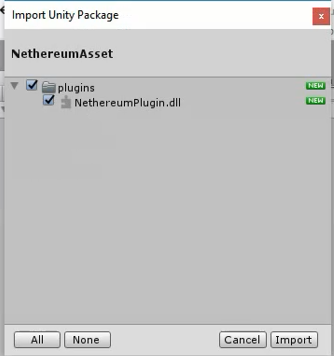
\includegraphics[width=10cm]{./unity3d-plugin/docs/image4.png}
\caption{\label{fig:orgb63ead7}
Opening the NethereumAsset package and importing objects.}
\end{figure}

\item After the installation is done, the plugin will be available inside the \texttt{plugins} folder that's been created.
\end{itemize}

\item Using Raw DLL

\begin{itemize}
\item Create a new folder called \texttt{plugins} inside the \texttt{Assets} folder of your Unity project.

\begin{figure}[htbp]
\centering
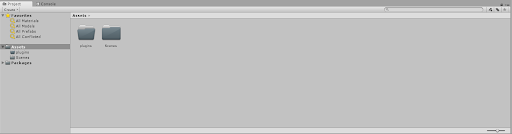
\includegraphics[width=10cm]{./unity3d-plugin/docs/image5.png}
\caption{\label{fig:org49a69ca}
Creating folder inside the Unity project directory.}
\end{figure}

\item Place the \textbf{\texttt{NethereumPlugin.dll}} inside the \texttt{plugins} folder.

\begin{figure}[htbp]
\centering
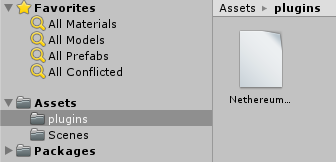
\includegraphics[width=10cm]{./unity3d-plugin/docs/image6.png}
\caption{\label{fig:org280810e}
Copying the plugin to the plugins folder.}
\end{figure}
\end{itemize}
\end{enumerate}

After finishing the plugin installation you must set now the .NET environment.

\begin{itemize}
\item On the top menu of Unity, select \texttt{Edit -> Project Settings -> Player}.
\item The inspector at the right will show several sections. Scroll to \texttt{Other Settings -> Configuration} and change the \texttt{Scripting Runtime Version} to \texttt{.NET 4.x Equivalent}. It will prompt you to restart Unity.

\begin{figure}[htbp]
\centering
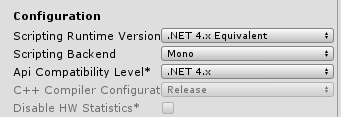
\includegraphics[width=10cm]{./unity3d-plugin/docs/image2.png}
\caption{\label{fig:orge1db561}
Changing the .NET environment.}
\end{figure}
\end{itemize}

\subsection{Plugin Usage}
\label{sec:orge521ee7}

Once the plugin has been correctly installed on your project, you can start using it. To do so, first you will have to create an instance of the plugin's class:

\begin{minted}[]{javascript}
var pluginInstance = new NethereumPlugin();
\end{minted}

\noindent
The instance will expose all the available methods for you to use.

\section{API Documentation}
\label{sec:org1a0d7cc}

This are the functionalities offered by the plugin.

\clearpage
\newgeometry{margin=1cm}
\begin{landscape}
\begin{longtable}{lllll}
\caption{\label{tab:orged6cd53}
API description.}
\\
Function Name & Description & Input & Input Description & Output\\
\hline
\endfirsthead
\multicolumn{5}{l}{Continued from previous page} \\
\hline

Function Name & Description & Input & Input Description & Output \\

\hline
\endhead
\hline\multicolumn{5}{r}{Continued on next page} \\
\endfoot
\endlastfoot
\hline
GenerateKeyPair & Method to retrieve the & None &  & Struct containing the public\\
 & public address and private &  &  & address and private key.\\
 & key. &  &  & \\
 &  &  &  & \\
DeepLink & Method to deep link to & - AppUri & Base URI of the app to communicate with. & None.\\
 & another application & - PublicAddress & Public address of your app. & \\
 &  & - TokenAddress & The ensName to be sent to other app. & \\
 &  & - Amount & Amount to be sent to other app. & \\
 &  & - ReturnLink & Callback method of your app. & \\
 &  &  &  & \\
InitUser & Creates a new user. & - URL & URL of the backend. & String containing the session token.\\
 &  & - IDFV & ID for vendor. & \\
 &  & - CoinId & ID of the coin to be use. & \\
 &  & - Amount & Amount of coin to initialize user. & \\
 &  &  &  & \\
UpdateUser & Updates the coin amount & - URL & URL of the backend. & None.\\
 & of user. & - Amount & Coin amount to be added or subtracted to user. & \\
 &  & - SessionToken & Session token received from InitUser. & \\
 &  &  &  & \\
GetUser & Retrieves the user coins & - URL & URL of the backend. & Returns the coin amount of the user.\\
 & amount given its session & - SessionToken & Session token received from InitUser. & \\
 & cookie. &  &  & \\
\end{longtable}

\end{landscape}
\restoregeometry
\end{document}
